\documentclass[12pt]{beamer}
\usetheme{default}
\usetheme{Boadilla}

\usepackage[utf8]{inputenc}
\usepackage[german]{babel}
\usepackage[T1]{fontenc}
\usepackage{amsmath}
\usepackage{amsfonts}
\usepackage{amssymb}
\usepackage{graphicx}
\usepackage{paralist}



\author{Quang-Long Pham}
\title{Webframework Django}
%\setbeamercovered{transparent} 
%\setbeamertemplate{navigation symbols}{} 
%\logo{
\includegraphics[scale=.05]{django-logo.png}} 
%\institute{} 
%\date{} 
%\subject{} 
\begin{document}

\begin{frame}
\titlepage
\end{frame}

%\begin{frame}
%\tableofcontents
%\end{frame}

\begin{frame}{Was ist Django?}

\begin{itemize}
	\item kostenlos
	\item open source
	\item Python Full-Stack-Framework 
	\item MVC und DRY Prinzip
	\item schnelle Entwicklung von \textbf{Web-Applikationen} 
	
	\end{itemize}
\end{frame}

\frame{
	\frametitle{Wer benutzt Django?}
	\begin{center} 
	\begin{inparaenum} 
	
	\item 
\includegraphics[scale=.2]{google.jpg} 
	
\includegraphics[scale=.2]{firefox-logo.png}
	
\includegraphics[scale=.2]{prezi.jpg}
	\item 
\includegraphics[scale=.2]{youtube-logo.png}
	
\includegraphics[scale=.3]{spotify-log.png}
	
\includegraphics[scale=.3]{pinterest-logo.png}
	
\includegraphics[scale=.2]{eve.png}
	
	\end{inparaenum}
	\end{center}
	}

\frame{
	\frametitle{Warum Django?}
	\begin{itemize}
	\item Python
	\item sehr steile Lernkuve
	\item auf allen OS benutzbar -> Editor
	\item sehr aktive Community, gute Dokumentation
	\item effiziente Grundstrukturen für die Entwicklung

	\end{itemize}
	}


\frame{
	\frametitle{Wie installiere ich Django?}
	\begin{exampleblock}
		{Installation} \$pip install Django
	\end{exampleblock}
	
	}
	
\frame{
	\frametitle{Wie benutze ich Django nun?}
		\begin{block}
		{Vorbereitung} \$django-admin\vspace{0.3cm}\\
		\hspace{1cm} check\\
		\hspace{1cm} cleanup\\
		\hspace{1cm} dumpdata\\
		\hspace{1cm} ...\\
		\hspace{1cm} shell\\
		\hspace{1cm} {\bf \color{orange} {runserver}\\
		\hspace{1cm} startproject\\
		\hspace{1cm} startapp\\}
		\hspace{1cm} syncdb\\
	\end{block}

	}
	
	\frame{
	\frametitle{Wie starte ich nun Django?}

	\begin{exampleblock}
		{Server starten} \$ python manage.py {\bf runserver}\vspace{0.3cm}\\
		\$ ls maddogProject\\
		Django version x.x.x, using settings 'maddogProject.settings'\\
		\vspace{0.3cm}Starting development server at http://127.0.0.1:8000\\
		Quit server with CONTROL-C\\
	\end{exampleblock} 
	
	}

	
	
\frame{
	\frametitle{Das erste Projekt erstellen}

	\begin{exampleblock}
		{Projektverzeichnis} \$ django-admin {\bf startproject maddogProject}						\vspace{0.3cm}\\
		\$ ls maddogProject\\
		{\bf \color{blue}maddogProject manage.py }\\
		\vspace{0.3cm}\$ ls -l maddogProject/maddogProject\\
		{\bf \_\_init\_\_.py\\
		settings.py \hspace{3cm}\\
		urls.py\\
		wsgi.py}
	\end{exampleblock} 
	
	}
	

\frame{
	\frametitle{Und jetzt?}

	\begin{exampleblock}
		{Browseraufruf!} 
		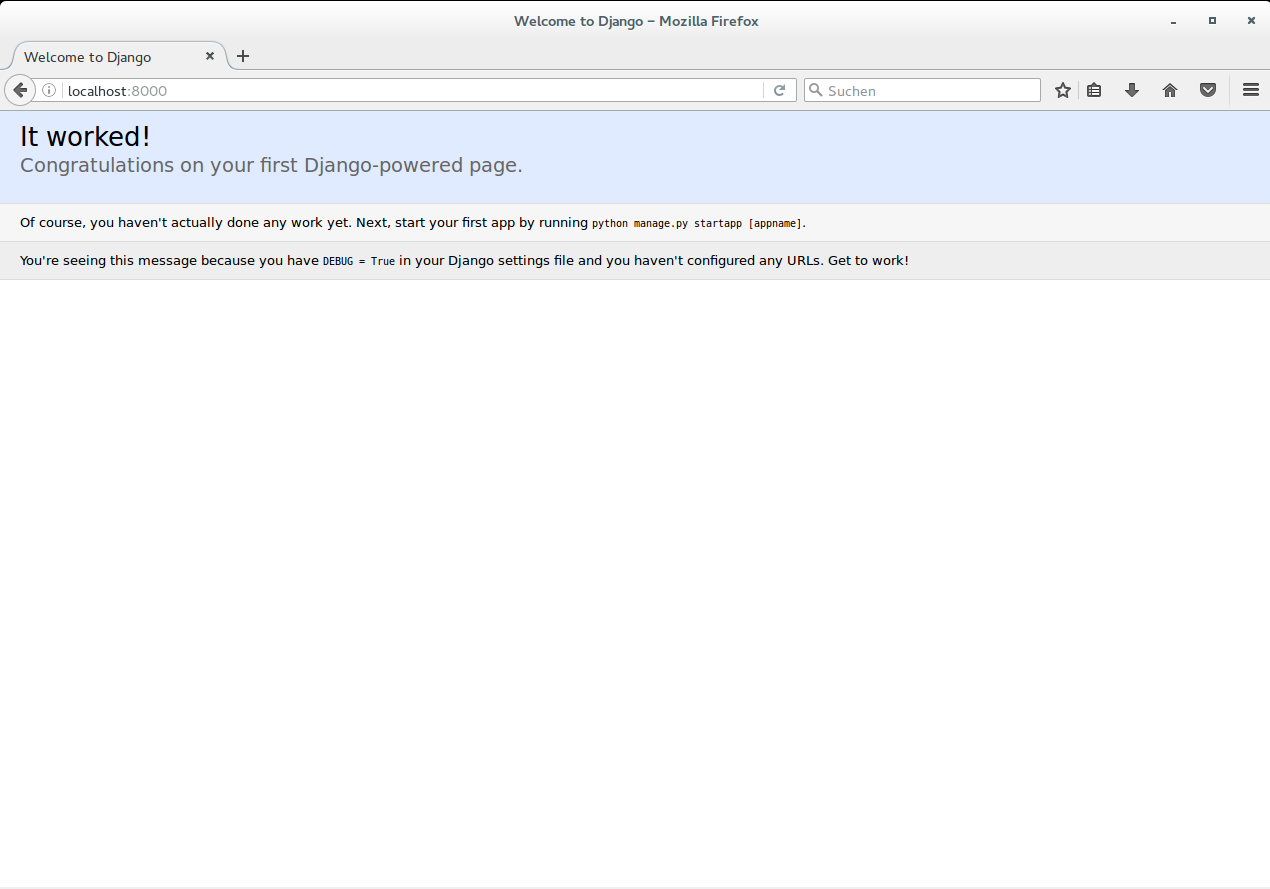
\includegraphics[scale=.3]{itworked.png}
	\end{exampleblock} 
	
	}		
	

\frame{
	\frametitle{Die erste Webseite erstellen}

	\begin{exampleblock}
		{Applikationsverzeichnis} \$ python manage.py {\bf startapp index}\vspace{0.3cm}\\
		\$ ls index\\
		{\bf \color{blue}maddogProject manage.py}\vspace{0.3cm}\\
		\$ ls -l maddogProject/maddogProject\\
		{\bf \_\_init\_\_.py\\
		admin.py\\
		models.py \hspace{3cm}\\
		tests.py\\
		views.py}
	\end{exampleblock}
	
	}



\frame{
	\frametitle{Django ist HTTP in, HTTP out!}
	\begin{center}
		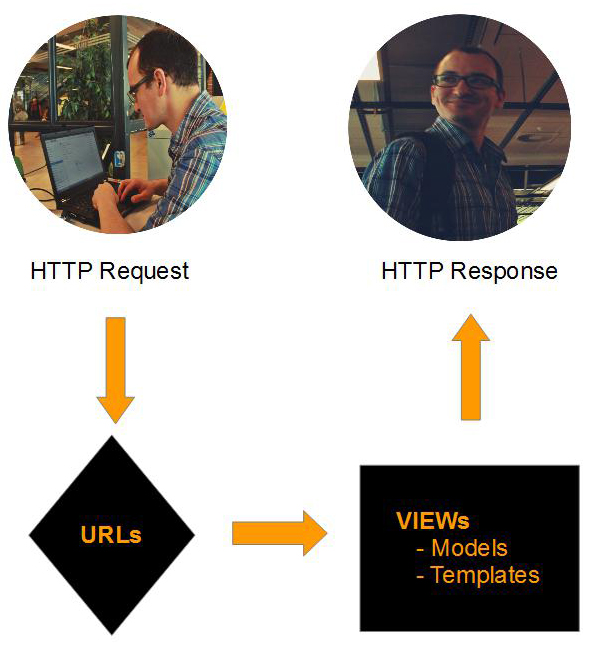
\includegraphics[width=0.55\textwidth]{MVC.jpg}
	\end{center}
	}

\frame{
	\frametitle{PyCharm}
	\begin{center}
	
		
\includegraphics[width=0.55\textwidth]{pycharm.png}\\
		https://www.jetbrains.com/pycharm/
	\end{center}
	}

\frame{
	\frametitle{Fragen?}
	\begin{center}
	
		Vielen Dank für Ihre Aufmerksamkeit!
		
	\end{center}
	}






\end{document}